\documentclass[preprint,12pt,3p,times]{elsarticle}
\biboptions{sort&compress}

%====package added by the authors
\usepackage[]{graphicx}
%\usepackage{float}
\usepackage{stackengine}
\usepackage{caption}
\usepackage{subfigure}
\usepackage{multirow}
\usepackage{amsmath,amssymb}
\usepackage{bm}
\usepackage{cases}
%\usepackage[round]{natbib}
\usepackage{booktabs}
\usepackage{soul,ulem}
\usepackage{setspace}
\usepackage[usenames, dvipsnames]{color}
\usepackage{lineno}
%\usepackage[nomarkers,tablesonly]{endfloat} % table managements
\usepackage[hidelinks]{hyperref} % for \url
\newcommand{\FS}[1]{{\textcolor{red}{\bf[FS: #1]}}}
\newcommand{\Mehdi}[1]{{\textcolor{OliveGreen}{\bf[Mehdi: #1]}}}
\newcommand{\rtwu}[1]{{\textcolor{blue}{\bf[#1]}}}
\newcommand{\rev}[1]{{\textcolor{blue}{#1}}}
%\renewcommand{\efloatseparator}{\vfill} % table managements
\soulregister\cite7
\soulregister\ref7
\soulregister\sout7
\soulregister\pageref7
\newcommand{\ed}[1]{{\textcolor{black}{#1}}}
\newcommand{\edit}[1]{{\textcolor{black}{#1}}}
\doublespacing
\DeclareRobustCommand{\hly}[1]{{\sethlcolor{yellow}\hl{#1}}}

\showboxdepth=\maxdimen
\showboxbreadth=\maxdimen


\begin{document}

\begin{frontmatter}

\title{Term Project: Using Computer Vision to Interpret Resistor Values}

\author[1]{Mugang Cho B11501160}

\address[1]{Department of Civil Engineering, National Taiwan University, Taipei, Taiwan}

\begin{abstract}
This report aims to explore a case study of utilizing computer vision in real-life applications: building a program that detects and interprets color codes on resistors. The primary goal is to find an efficient method that accurately identifies the color bands on the resistor. The program will then calculate the resistance value based on what it identified. Overall, the research demonstrates a method that can automate and streamline the resistor identification process, reducing human error and enhancing productivity in electronic component handling.
\end{abstract}

\begin{keyword}
Computer Vision \sep Resistor Color Code \sep Image Processing \sep Computer Vision \sep Object Detection \sep Electronic Components

\end{keyword}
    
\end{frontmatter}

\section{Introduction}
In electronic circuits, resistors regulate the electric current by its resistance. The value of the resistance is represented by a series of color bands printed on the resistor. Traditionally, the methods for resistor identification involved manual inspection or basic electronic testing equipment. However, the current state-of-the-art methods include computer vision and machine learning techniques. This research will trace specifically how these techniques work. Our approach involves image preprocessing, color segmentation, and possibly convolutional neural networks to ensure high accuracy under vast conditions. 

\subsection{Motivation and Relevant Works}
In \cite{ref1}, the authors have a similar objective to this paper. However, its approach is to recognize the colors in real-time video analysis. The key ideas to be taken are color space transformation and color extraction. The authors converted RGB color space to HSV color space to simplify the mixture of colors that may come from other variants. As for the extraction, the authors implemented a self-developed method that detects the colors in a moving frame.
In \cite{ref2}, the authors proposed an enhanced segmentation method by implementing feature extraction of three-dimensional parameter color images and edge and corner-detecting algorithms.

\subsection{Contribution and Scope}
This research practically contributes to the field by:
\begin{itemize}
\item assisting electrical engineering students via integrating the program into the mobile apps.
\item verification in the work field.
\end{itemize}
It also provides insight into how machine learning and computer vision are implemented.
The scope of this study includes the design, implementation, and evaluation of the proposed system, along with a discussion of potential improvements and future research directions.

\section{Datasets}
The datasets used in this research consist of images capturing 67 distinct values of 4-band resistors and 60 distinct values of 5-band resistors, all taken using a USB microscope \cite{ref3}. The images are taken against five different backgrounds: wood, white paper, yellow notepad, book cover, and book page. Additionally, resistors are photographed with two different leg orientations: bent and straight. The purpose of these varied datasets is not to train the model (as our approach does not rely on deep learning), but to thoroughly evaluate the model's performance under diverse conditions. Figure \ref{f_resistors} illustrates one of the images from the dataset.

\begin{figure}[!h]
    \centering
    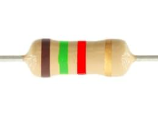
\includegraphics[width=0.8\textwidth]{resistor3.png}
    \caption{\label{f_resistors}The color codes on the body of an example resistor.}
\end{figure}

\section{Methodology}\label{s_method}
The fundamental aspect of calculating the resistance value is the order of the color code. For instance, for a 4-band resistor, the first and second bands represent the significant figures, the third band represents the multiplier, and the last band represents the tolerance percentile \cite{ref4}. For this reason, it is crucial to accurately identify the color codes on resistors in their correct order. Table \ref{t_data_stats} shows the values of the color codes.

\begin{table}[!h]
    \centering
    \caption{\label{t_data_stats}Resistor color code values}
    \begin{tabular}{|l|l|l|l|}
    \hline
    \textbf{Color} & \textbf{Value} & \textbf{Multiplier} & \textbf{Tolerance} \\ \hline
    Black          & 0              & 1                   &                   \\ \hline
    Brown          & 1              & 10                  & 1\%               \\ \hline
    Red            & 2              & 100                 & 2\%               \\ \hline
    Orange         & 3              & 1k                  & 3\%                 \\ \hline
    Yellow         & 4              & 10k       
              & -0, +100\%               \\ \hline
    Green          & 5              & 100k                & 0.5\%             \\ \hline
    Blue           & 6              & 1M                  & 0.25\%            \\ \hline
    Violet         & 7              & 10M                 & 0.1\%             \\ \hline
    Gray           & 8              & 100M                & 0.05\%            \\ \hline
    White          & 9              & 1G                  & 10\%                  \\ \hline
    Gold           &                & 0.1                 & 5\%               \\ \hline
    Silver         &                & 0.01                & 10\%              \\ \hline
    \end{tabular}
    \end{table}

\subsection{Primary Methodology}
Our methodology begins by rotating the image so that the color codes are oriented vertically, aligning with the direction in which the machine reads the pixels. This alignment ensures consistent and accurate color detection.
Next, the program sequentially detects the individual colors, continuing this process until it encounters a change in color. This detection can be achieved through two primary methods: converting the image from RGB to the HSV color space \ref{ref2}, which simplifies color differentiation, or employing a Convolutional Neural Network (CNN) specifically trained to identify resistor colors with high precision.
Once the program has successfully identified all the color bands, it calculates the resistance value using the standard color code formula.

\begin{equation}
    \label{eq_resistor}
    R = (10 \times \text{band1} + \text{band2}) \times \text{band3}
\end{equation} 

\subsection{Refined Methodology}
As we found deficiencies while developing the program for the primary methodology, we propose a more plausible approach that involves the following steps:
\begin{enumerate}
	\item Edge detection: Detect the edges of the resistor to find the center line.
	\item Center line detection: Locate the center line of the resistor to crop the image.
	\item Image cropping: Crop the image to focus on the resistor body. (Done manually in this research, but can be automated in future work.)
	\item Color detection: Detect the colors on the resistor body to identify the color codes.

\end{enumerate}
The biggest reason why we decided to refine the methodology is due to our ignorance of the background color. The program was not designed to adapt in such conditions. Therefore, we had to pick the images that had clean and white background so that it could extract the color codes. Only under this condition, the refined program depicts the accurate resistance value.

To get into further details, the method used for the edge detection is the Canny edge detection algorithm. First, it removes the noise of the image by 5x5 Gaussian filter. Then, it calculates the edge gradient using the Sobel operator. 	 
\begin{equation}
	\label{eq_edge}
	G = \sqrt{G_x^2 + G_y^2}
\end{equation}
\begin{equation}
	Angle = \arctan{\frac{G_y}{G_x}}
\end{equation}
Using the given magnitude and direction of the edge gradient, the algorithm detects every pixel that is normal to the gradient. The detected pixels are then connected to form the edges of the resistor. \cite{ref5}

The center line detection is done by Hough line detection algorithm \cite{ref6}. The algorithm detects the lines that pass through the most number of edge pixels using the following formula:
\begin{equation}
	\label{eq_hough}
	r = x \cos{\theta} + y \sin{\theta}
\end{equation}
This method is convenient for detecting the resistor, because the shape of the resistor is symmetric, and the center line is always located in the middle of the resistor. This way, the color bands are always located in the same position.

Finally, the color codes are detected by converting the image to the HSV color space \cite{ref1}. The program then detects the colors by setting the range of the hue values. The detected colors are then compared to the color code values in Table \ref{t_data_stats} to calculate the resistance value. Here, we implement the algorithm that if the Hue value of the pixel is within the range of the color code of the list in Table \ref{t_data_stats}, the program will detect the color. 

\section{Results and Discussions}\label{s4}
The program was initially tested on one high quality image from the dataset. The image was taken against a white background, and the resistor was oriented straight.

Edge detection was performed, the results can be seen in Figure \ref{f_edge}. The program successfully detected the edges of the resistor, which allowed for the center line to be detected. 

The center line detection results are shown in Figure \ref{f_center}. The program detected the center line of the resistor, which was then used to crop the image. The cropped image is shown in Figure \ref{f_cropped}.

The color detection was then attempted without success. The program was unable to reliably detect contiguous color bands on the resistor body. This failure was attributed to the program's inability to adapt to the variations in hue and saturation values caused by the lightning. The results produced by the program are shown in Figure \ref{f_color}. Consequently, band calculation produced incorrect results.

\begin{figure}[!h]
    \centering
    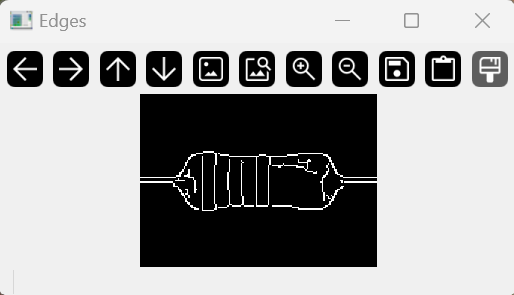
\includegraphics[width=0.8\textwidth]{screen2.png}
    \caption{\label{f_edge}Edge detection results.}
\end{figure}

\begin{figure}[!h]
    \centering
    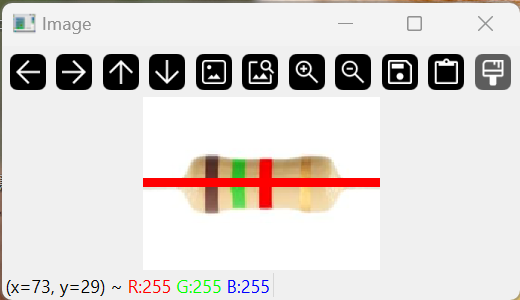
\includegraphics[width=0.8\textwidth]{screen3.png}
    \caption{\label{f_center}Center line detection results.}
\end{figure}

\begin{figure}[!h]
    \centering
    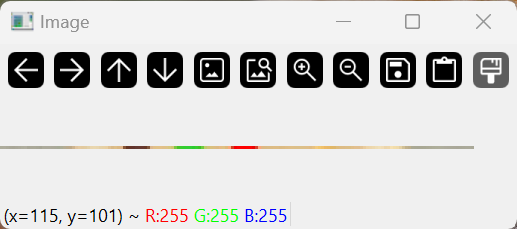
\includegraphics[width=0.8\textwidth]{screen4.png}
    \caption{\label{f_cropped}Cropped image results.}
\end{figure}

\begin{figure}[!h]
    \centering
    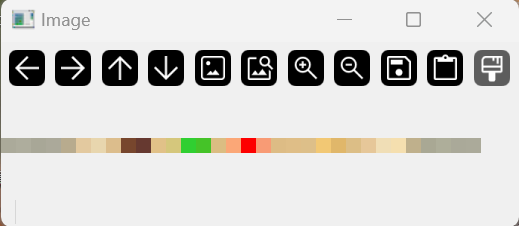
\includegraphics[width=0.8\textwidth]{screen5.png}
    \caption{\label{f_color}Color detection results.}
\end{figure}

\subsection{Discussion}
The program's failure to detect the color codes accurately can be attributed to the following factors:
\begin{itemize}
    \item The program was not designed to adapt to variations in hue and saturation values caused by the lightning.
    \item The program was not trained to detect color codes in different backgrounds.
    \item The program was not trained to detect color codes in different resistor orientations.
\end{itemize}

\subsection{Future Work}
To improve the program's performance, the following could be implemented:
\begin{itemize}
    \item As the program failed at the color detection stage, the program could be trained to detect color codes in different backgrounds and resistor orientations. A CNN trained with color bands in different environments can be utilized for this purpose.
    \item Orientation detection could be implemented to automatically rotate the image to align the color bands vertically.
\end{itemize}

\section{Conclusion}\label{s5}
The research shows unexpected variables may cause the program to fail drasitically. We had to put many threshholds. Therefore it did not turn out as an ideal result.

This research has also shown the usability of deep learning in computer vision. Some tasks could be simplified by using deep learning. The program could be trained to detect color codes in different backgrounds and resistor orientations, instead of relying on manual thresholding.

Our current program predominantly operates without deep learning methods, utilizing such techniques only minimally for tasks like color detection. For future research, I propose experimenting with inputting raw resistor data directly into a convolutional neural network (CNN) and comparing the results with those obtained from the current program. This comparison aims to determine whether the CNN-based approach offers superior accuracy over the numerical and rigid formula-based methods currently in use. Additionally, I am interested in expanding the application of this technology to other scenarios requiring precise color detection and identification.

The updated source code is available at \url{https://github.com/mugangcho1234/dl-term-resistors}.

\section{Acknowledgment}\label{s6}
The author would like to thank the Department of Civil Engineering at National Taiwan University for providing the valuable opportunity to conduct this research. The challenges faced during this project have enhanced problem-solving skills, especially as a beginner in report writing. Additionally, thanks to the anonymous reviewers for their valuable feedback.


\bibliographystyle{unsrt}
\bibliography{references}

\end{document}

